\bigskip
\section{Evaluate and Summarize Your Results}\label{sec:trace}

%TODO some text here
% what is interesting? What are we looking for? 

\medskip
\subsection{Evaluate MCMC}\label{subsub:Exercise-EvalMCMC}

As discussion in \cl{RB\_Total\_Evidence\_TEFBD}, we will use Tracer to evaluate the MCMC samples from our three estimations. 
Load all three of the MCMC logs into the Tracer window.
The MCMC chains will not have converged because they have not been run very long. 
Highlight all three files in the upper left-hand viewer (Fig. \ref{fig:tracer-files}) by right- or command-clicking all three files.

\begin{figure}[h!]
\fbox{%
\begin{minipage}{\textwidth}\centering
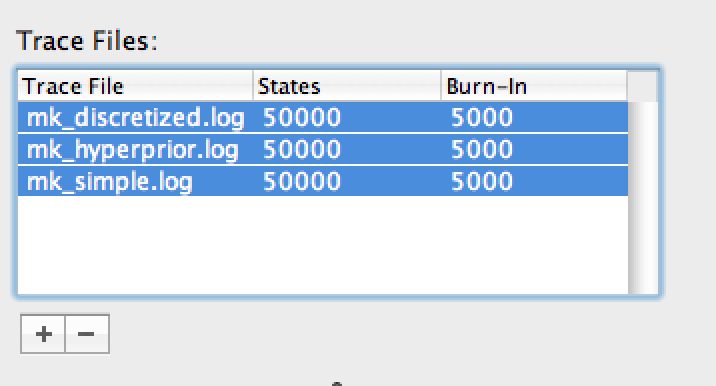
\includegraphics[width=0.5\textwidth,angle=0]{\ResourcePath figures/AddFiles}
\caption{\small Highlight all three files for model comparison.}
\end{minipage}}
\label{fig:tracer-files}
\end{figure}

Once all three trace logs are loaded and highlighted, first look at the estimated marginal likelihoods.
You will notice that the Mk model, as originally proposed by \citep{lewis01} is improved by allowing any state frequency heterogeneity at all. 
The discretized model and the Dirichlet model both represent improvements, but are fairly close in likelihood score to each other (Fig. \ref{fig:tracer-llik}).
Likely, we would need to perform stepping stone model assessment to truly tell if the more complicated model is statistically justified.
This analysis is too complicated and time-consuming for this tutorial period, but you will find instructions below for performing the analysis. \par
\begin{figure}[h!]
\fbox{%
\begin{minipage}{\textwidth}\centering
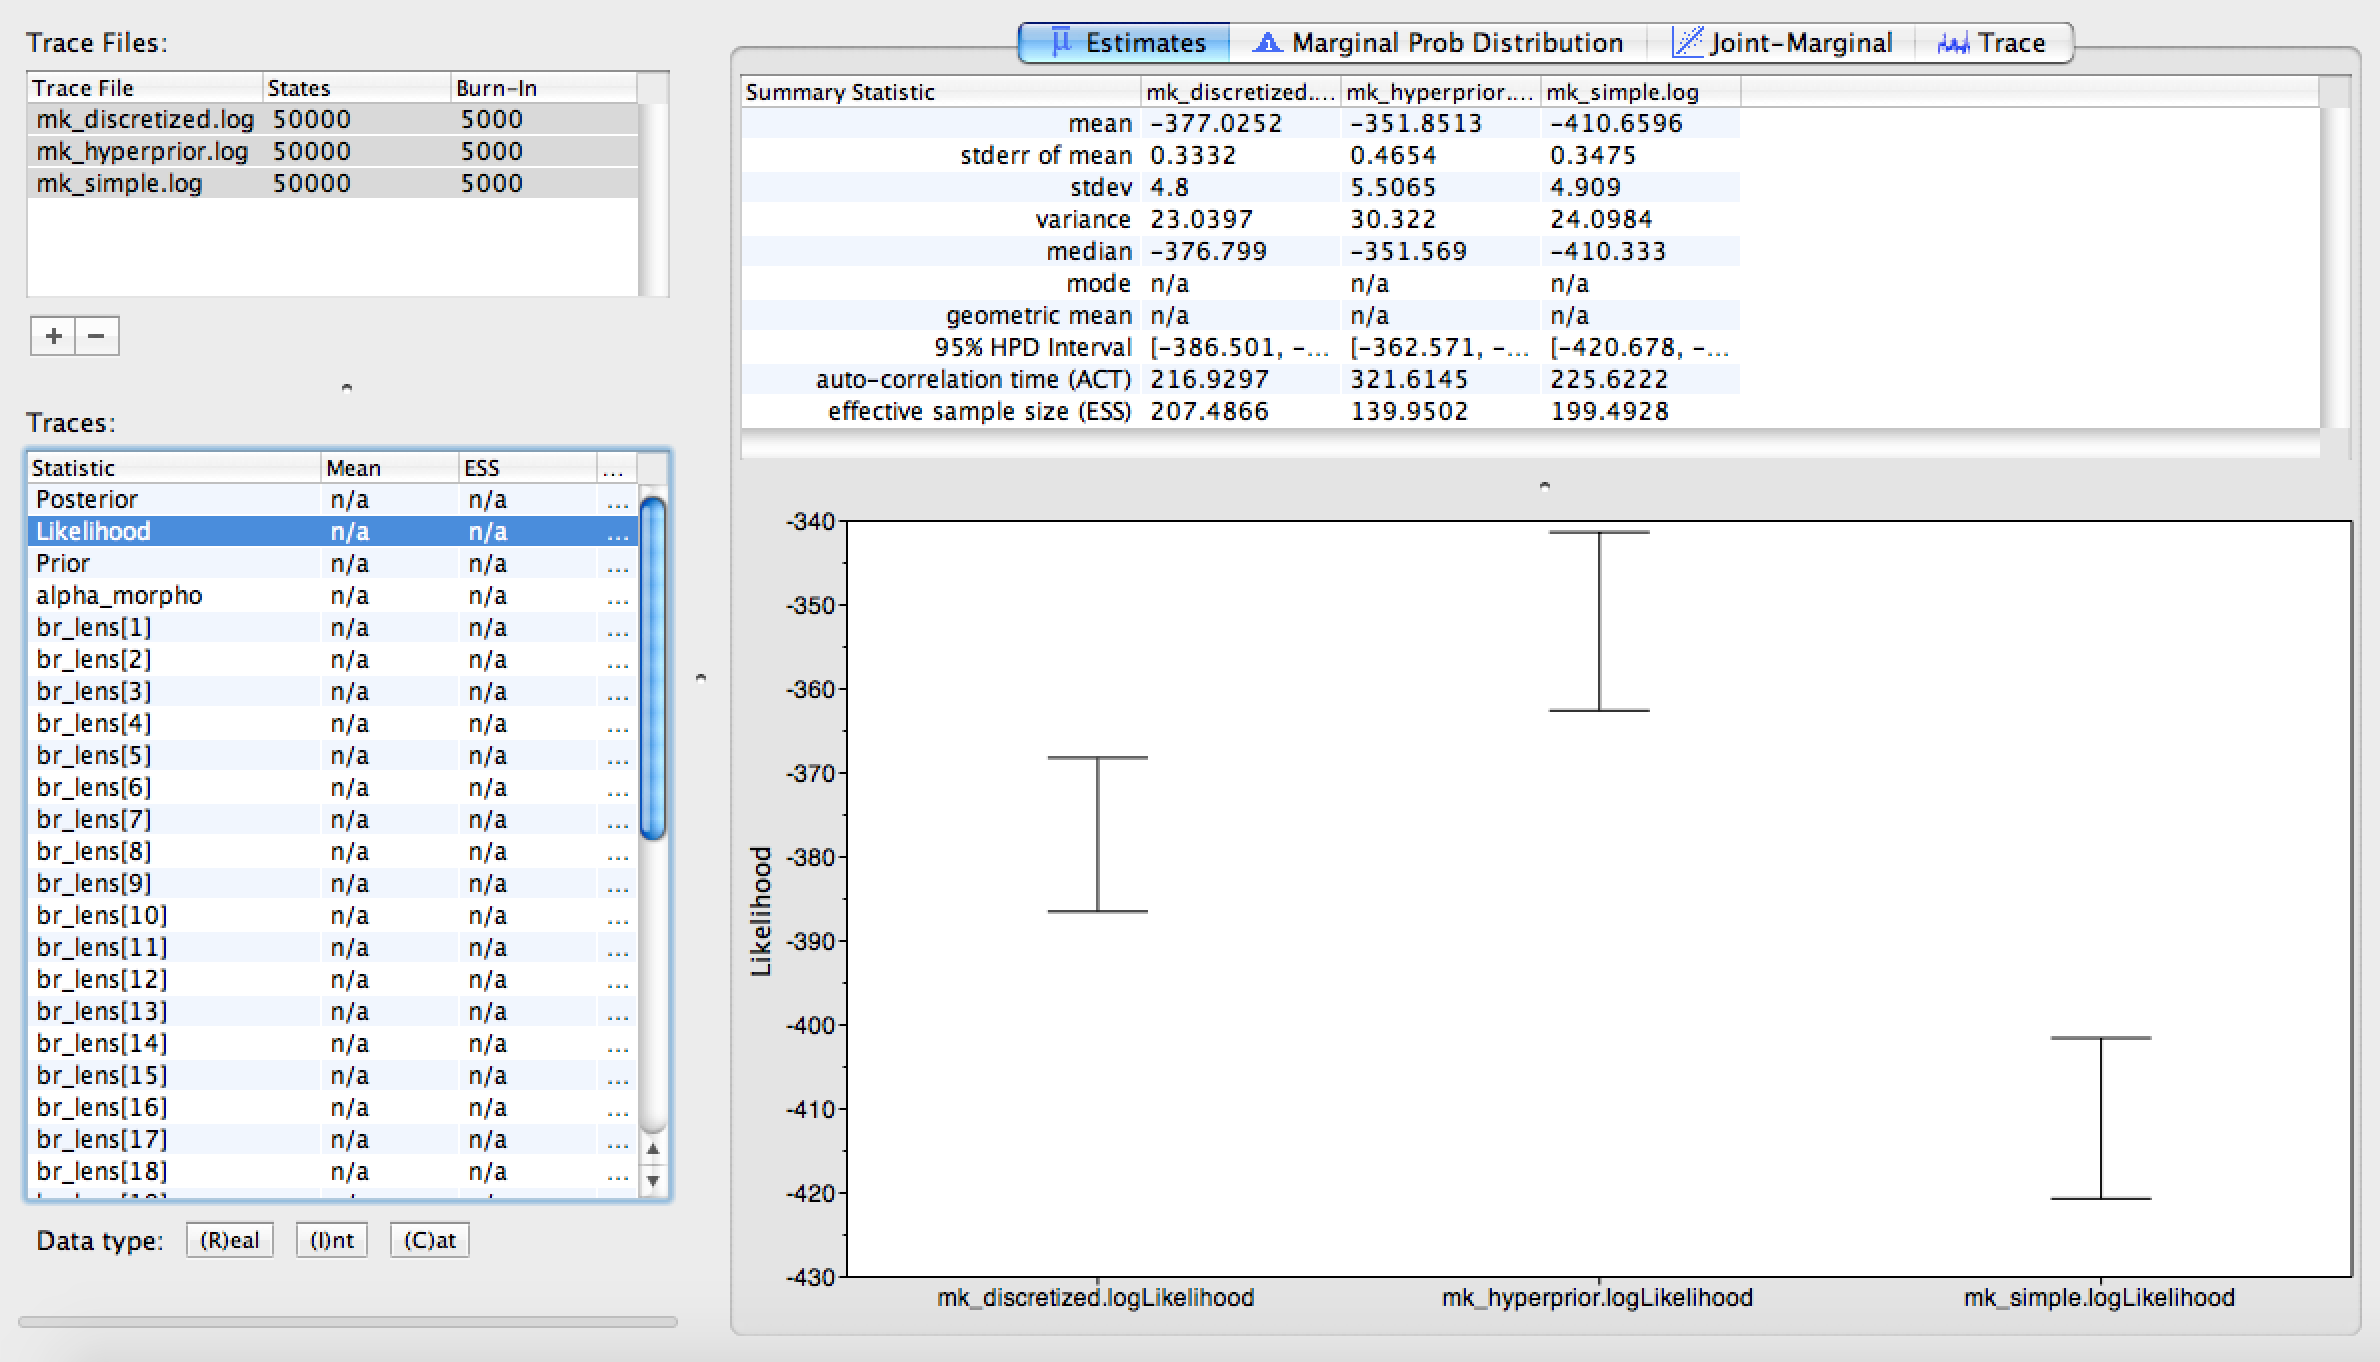
\includegraphics[width=0.75\textwidth,angle=0]{\ResourcePath figures/likelihoods}
\caption{\small Comparison of likelihood scores for all three models.}
\end{minipage}}
\label{fig:tracer-llik}
\end{figure}

Click on the `Trace' panel.
In the lower left hand corner, you will notice an option to color each trace by the file it came from.
Choose this option (you may need to expand the window slightly to see it).
Next to this option, you can also see an option to add a legend to your trace window.
The results of this coloring can be seen in Fig. 6.
When the coloring is working, you will see that the Mk model mixes quite well, but that mixing becomes worse as we relax the assumption of equal state frequencies.
This is because we are greatly increasing model complexity.
Therefore, we would need to run the MCMC chains longer if we were to use these analyses in a paper. \par

\begin{figure}[h!]
\fbox{%
\begin{minipage}{\textwidth}\centering
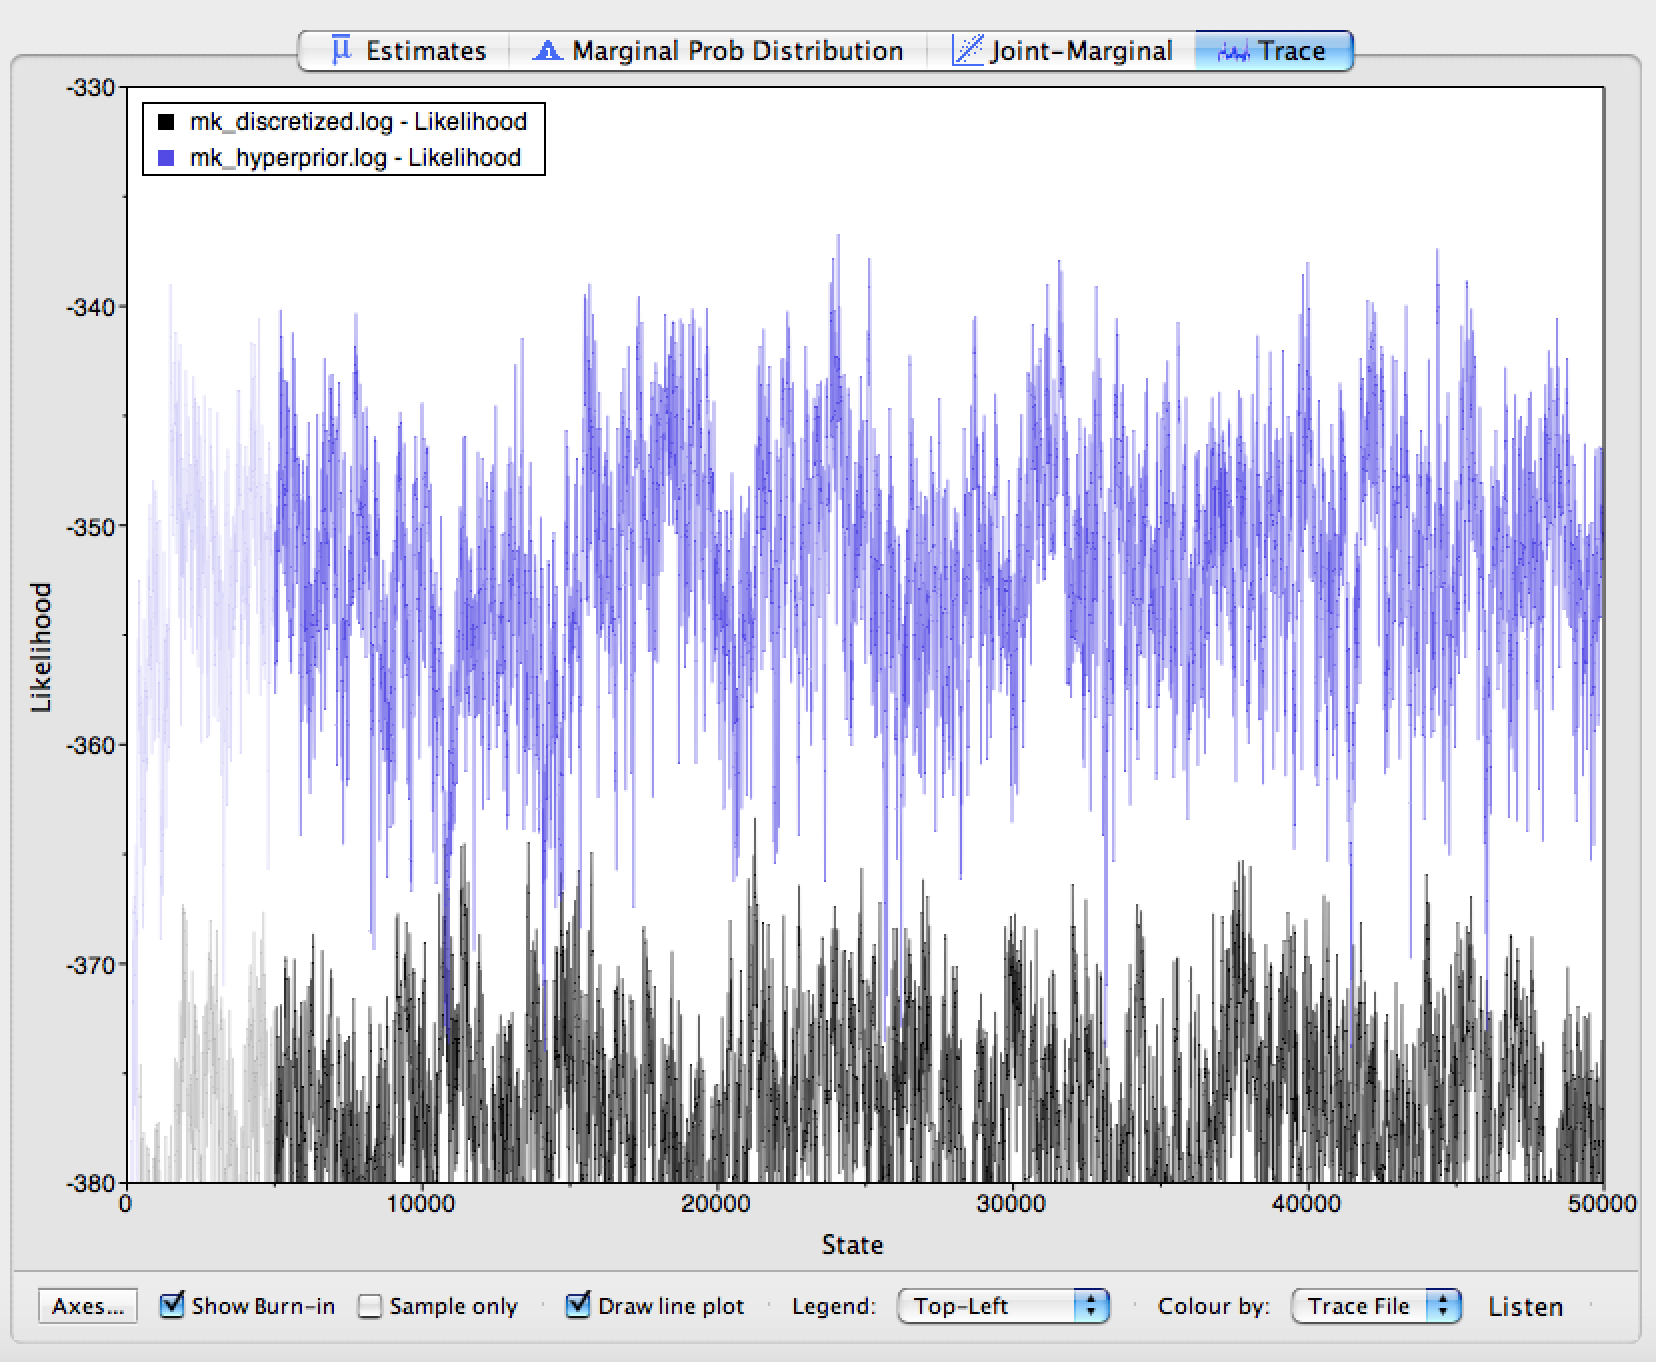
\includegraphics[width=0.6\textwidth,angle=0]{\ResourcePath figures/colortrace}
\caption{\small The Trace window. The traces are colored by which version of the Mk model they correspond to.}
\end{minipage}}
\label{fig:module-gm}
\end{figure}


We are interested in two aspects of the posterior distribution.
First, all analyses correct for the biased sampling of variable characters except for the {\tt simple} analysis.
Then, we expect the {\tt tree\_length} variable to be greater for {\tt simple} than for the remaining analyses, because our data are enriched for variation.
Figure \ref{fig:tracer_tree_length} shows that {\tt tree\_length} is approximately 30\% greater for {\tt simple} than for {\tt mk\_simple}, which are identical except that {\tt mk\_simple} corrects for sampling bias.
To compare these densities, click the ``Marginal Prob Distribution'' tab in the upper part of the window, highlight all of the loaded Trace Files, then select {\tt tree\_length} from the list of Traces.

\begin{figure}[h!]
\fbox{%
\begin{minipage}{\textwidth}\centering
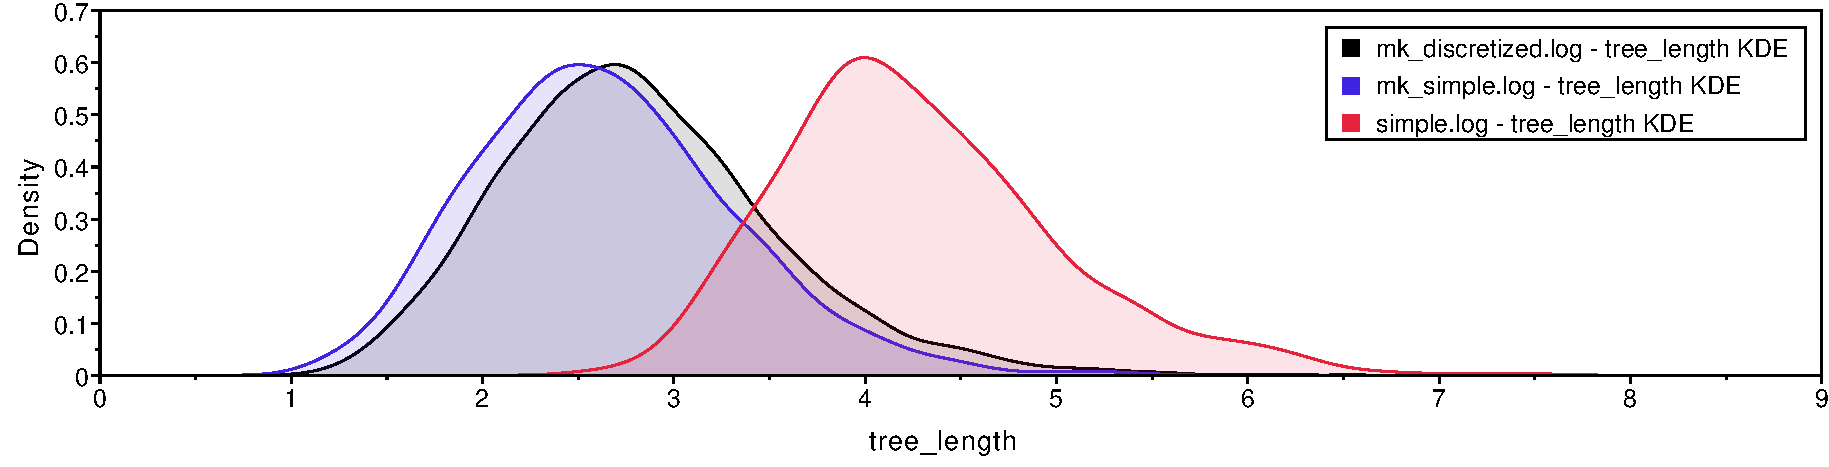
\includegraphics[width=0.9\textwidth,angle=0]{\ResourcePath figures/results/tracer_tree_length}
\caption{\small Posterior tree length estimates.}
\end{minipage}}
\label{fig:tracer_tree_length}
\end{figure}

Second, we are interested in characterizing the degree of heterogeneity estimated by the beta-discretized model.
If the data were distributed by a single morphological rate matrix, then we would expect to see very little variation among the different values in {\tt cats}, and very large values for the shape and scale parameters of the discrete-beta distribution.
For example, if {\tt alpha\_ofbeta = beta\_ofbeta = 1000}, then that would cause all discrete-beta categories to have values approaching 0.5, which approximates a symmetric Mk model.

\begin{figure}[h!]
\fbox{%
\begin{minipage}{\textwidth}\centering
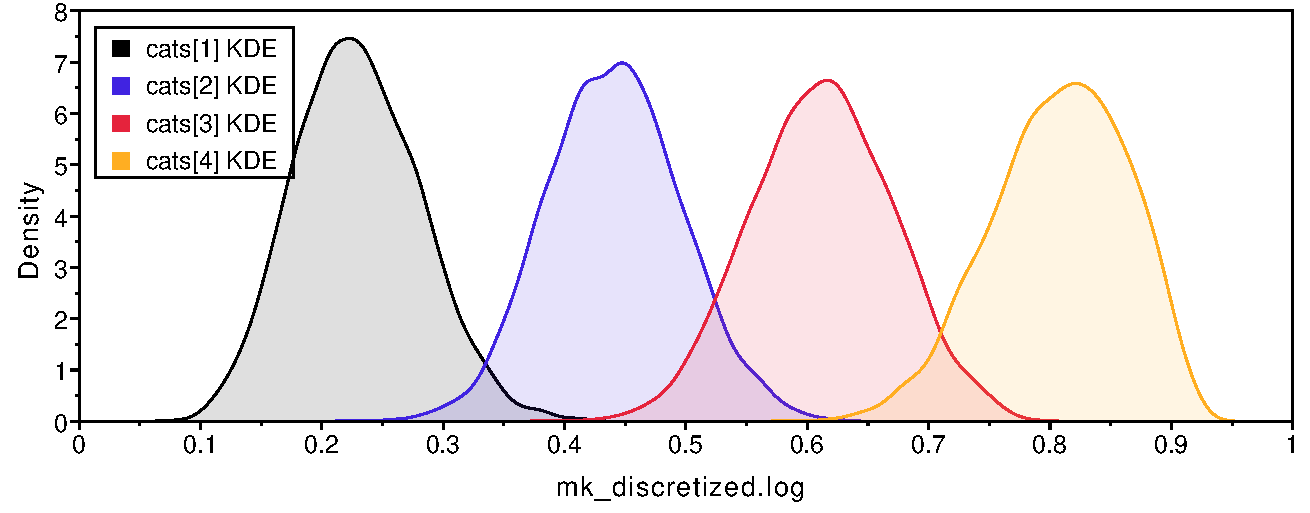
\includegraphics[width=0.9\textwidth,angle=0]{\ResourcePath figures/results/cats}
\caption{\small Posterior tree length estimates.}
\end{minipage}}
\label{fig:tracer_cats}
\end{figure}

\begin{figure}[h!]
\fbox{%
\begin{minipage}{\textwidth}\centering
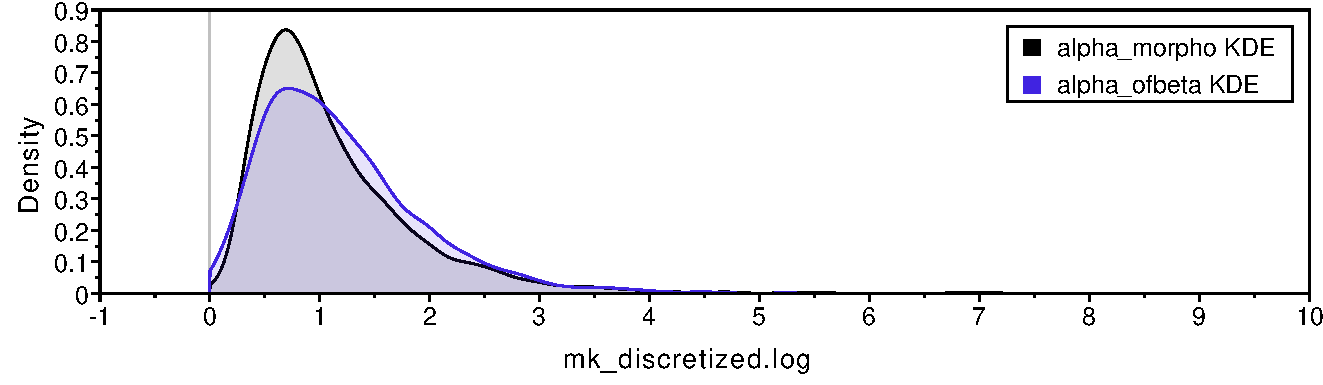
\includegraphics[width=0.9\textwidth,angle=0]{\ResourcePath figures/results/alpha_beta}
\caption{\small Posterior tree length estimates.}
\end{minipage}}
\label{fig:tracer_alpha_beta}
\end{figure}

Figure \ref{fig:tracer_cats} shows that the four discrete-beta state frequencies do not all have the exact same value.
In addition, Figure \ref{fig:tracer_alpha_beta} shows that the priors on the discrete-beta distribution are small enough that we expect to see variance among {\tt cat} values.
If the data contained no information regarding the distribution of {\tt cat} values, then the posterior estimates for {\tt alpha\_ofbeta} and {\tt beta\_ofbeta} would resemble the prior.

\subsection{Summarizing tree estimates}

\begin{figure}[h!]
\fbox{%
\begin{minipage}{\textwidth}\centering
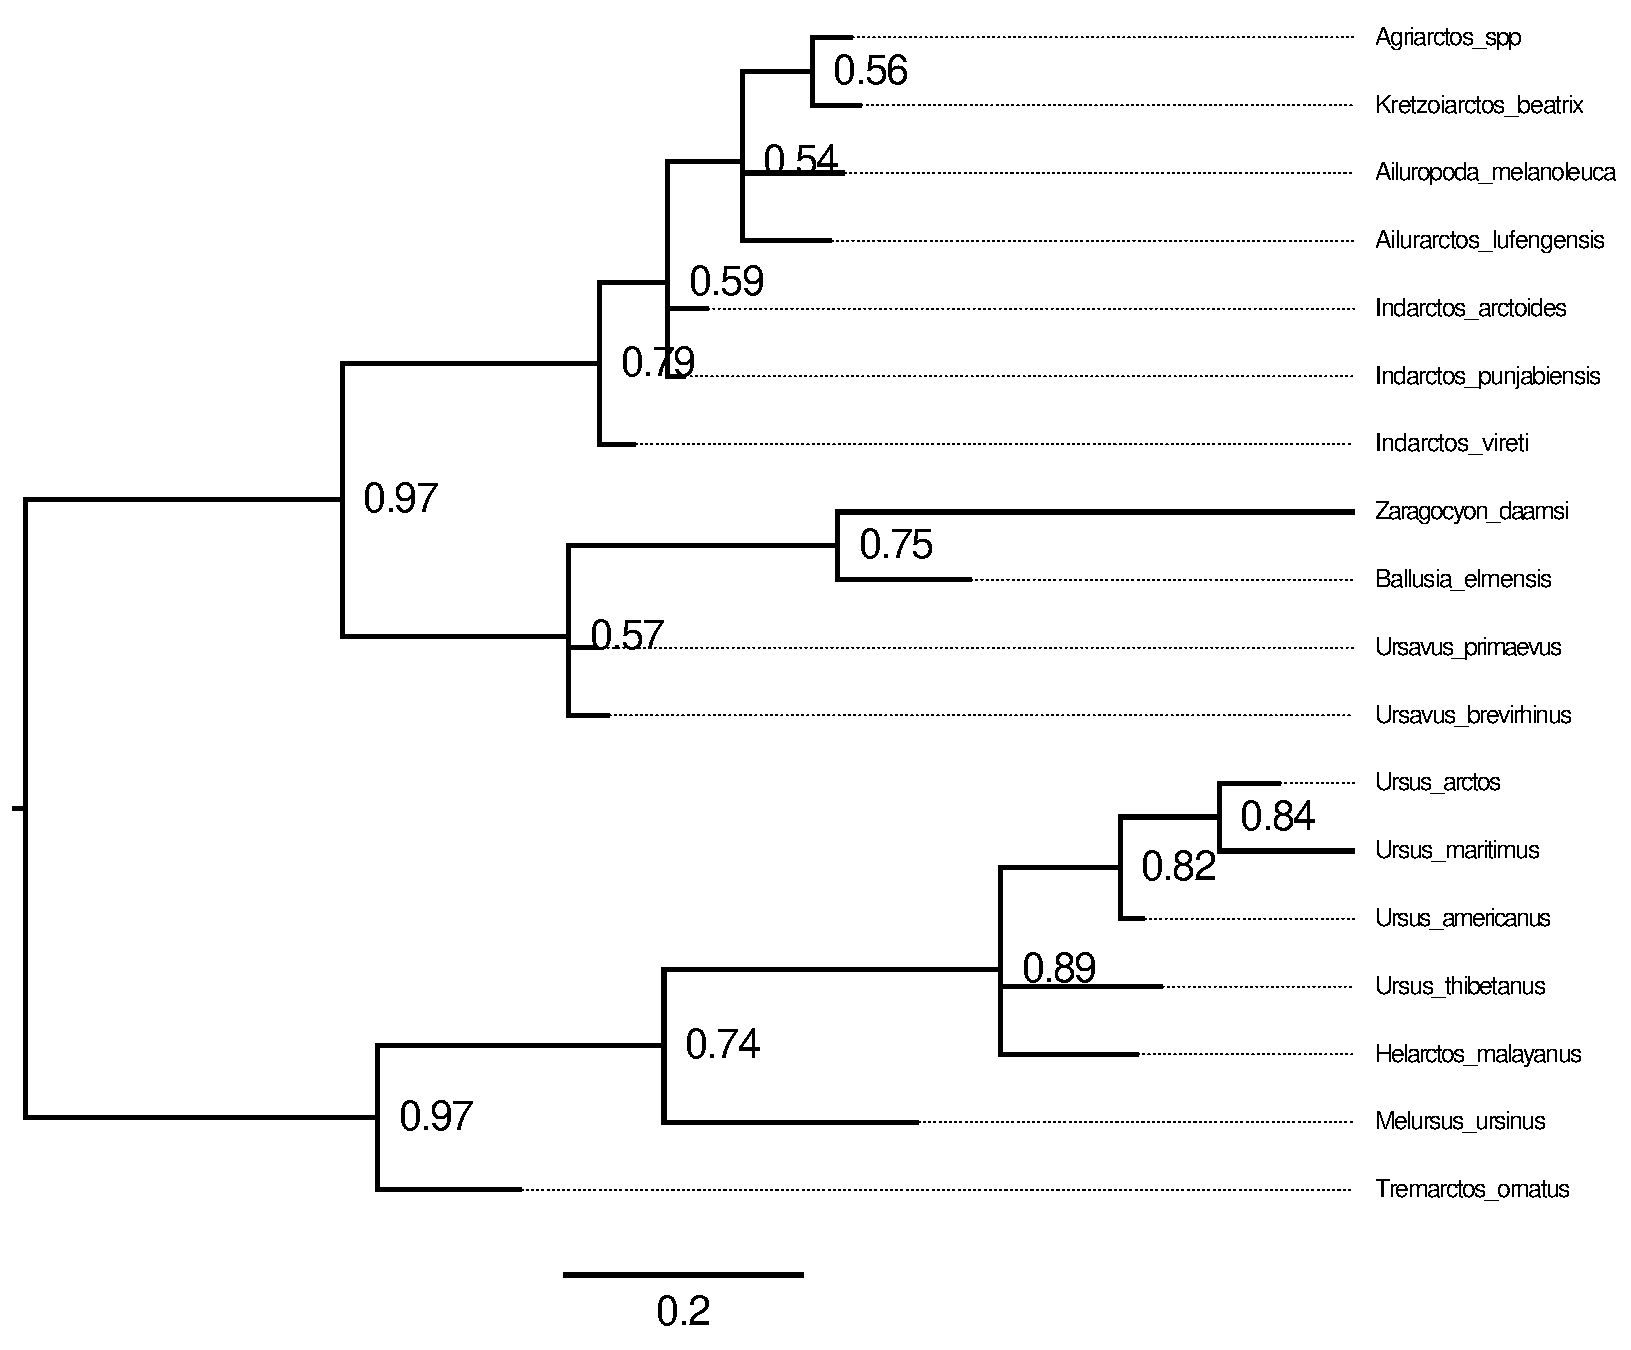
\includegraphics[width=0.6\textwidth,angle=0]{\ResourcePath figures/results/simple_majrule_tre}
\caption{\small Majority rule consensus tree for the uniform Mk analysis.}
\end{minipage}}
\label{fig:simple_majrule}
\end{figure}


The morphology trees estimated in \ref{sec:dm_simple} and \ref{sec:dm_disc} are summarized using a majority rule consensus tree (MRCT).
Clades appearing in $p>0.5$ of posterior samples are resolved in the MRCT, while poorly support clades with $p \leq 0.5$ are shown as unresolved polytomies.
%Poor support for clades is typically caused by either having too little  conflicting phylogenetic information.
Poor phylogenetic resolution might be caused by having too few phylogenetically informative characters, or it might be due to conflicting signals for certain species relationships.
Because phylogenetic information is generated through model choice, let's compare our topological estimates across models.

\begin{figure}[h!]
\fbox{%
\begin{minipage}{\textwidth}\centering
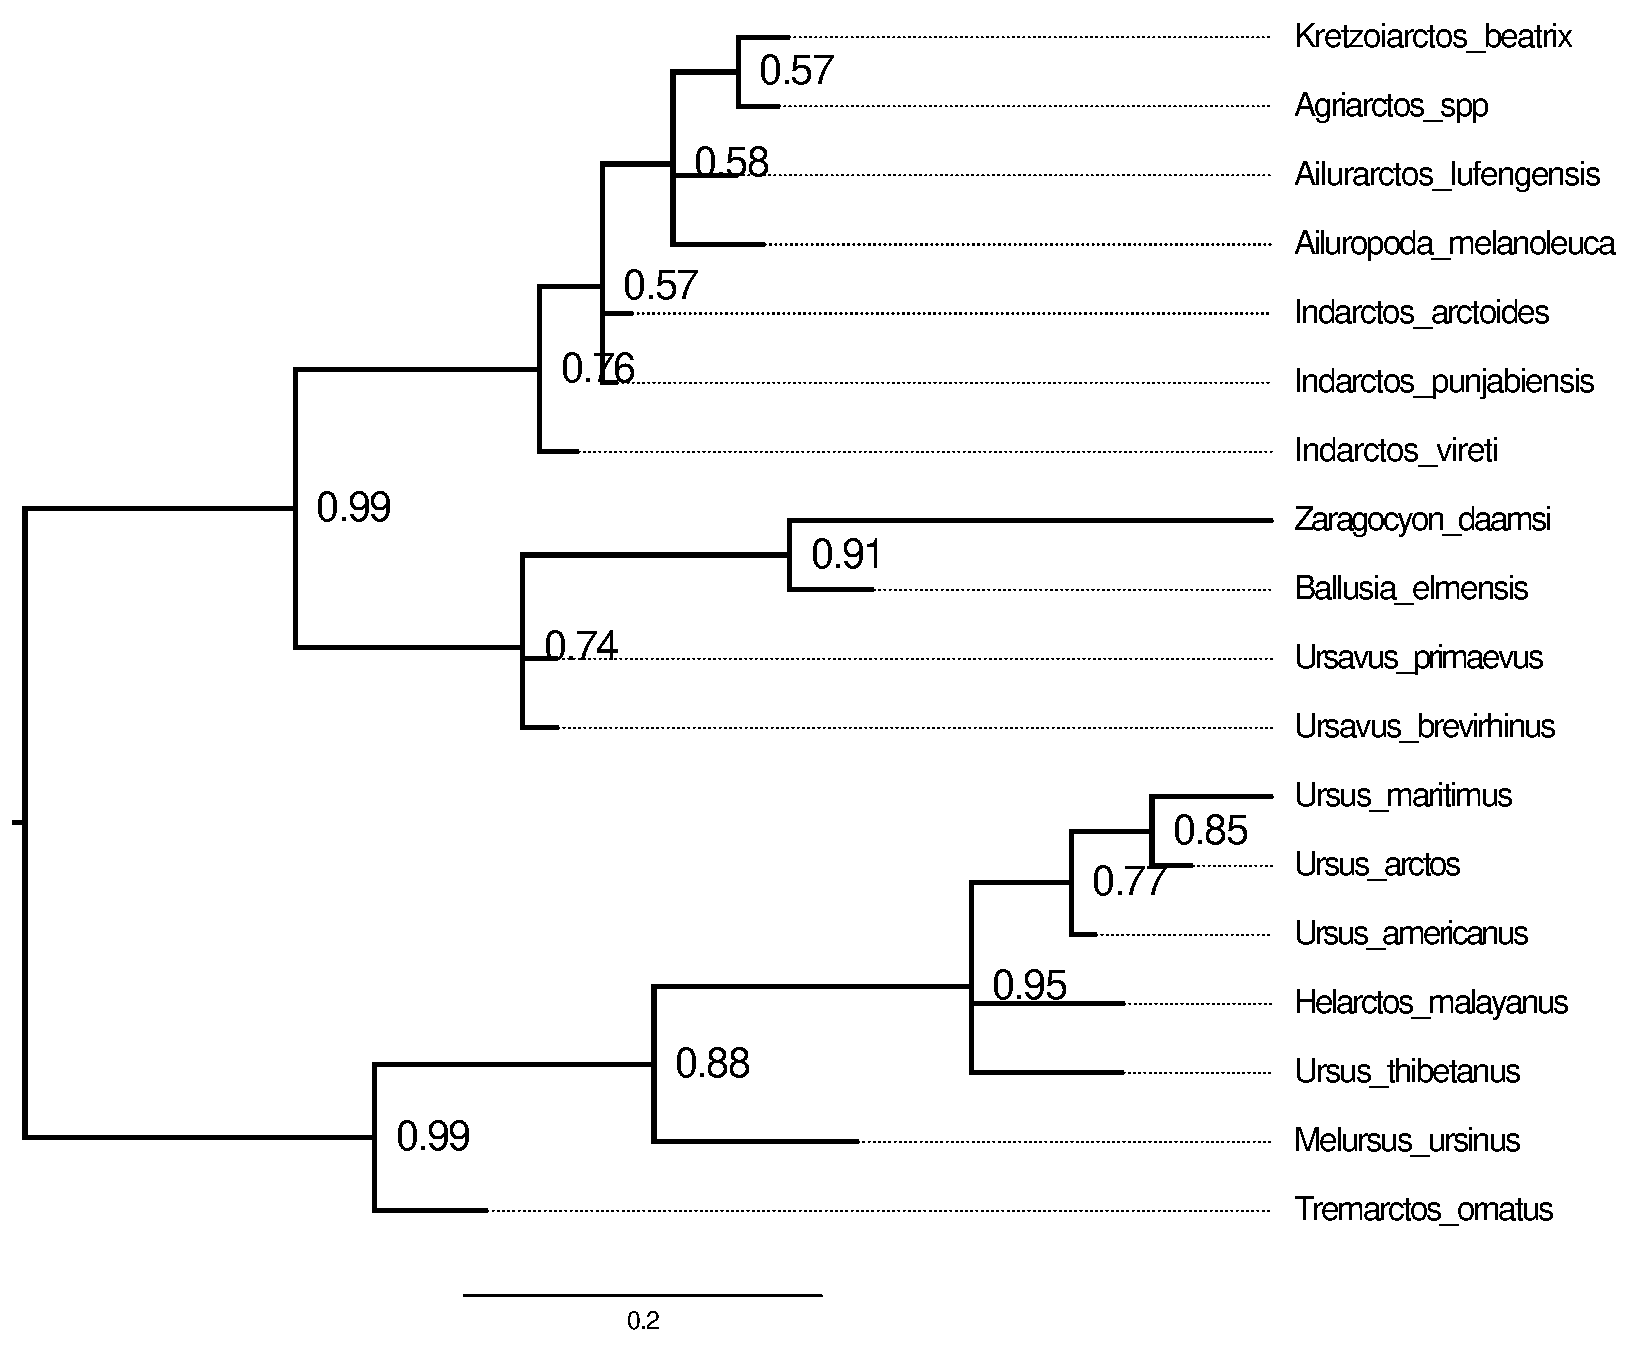
\includegraphics[width=0.6\textwidth,angle=0]{\ResourcePath figures/results/mk_discretized_majrule_tre}
\caption{\small Majority rule consensus tree for the beta-discretized Mkv analysis.}
\end{minipage}}
\label{fig:mk_discretized_majrule}
\end{figure}

The MRCTs for the simple model without the +v correction (Fig \ref{fig:simple_majrule}) and the discretized-beta model (Fig \ref{fig:mk_discretized_majrule}) produce trees with comparable support for clades.
Note that the scale bars for branch lengths differ greatly, indicating that tree length estimates are inflated without the +v correction, just as we saw when comparing the posterior tree length densities.
In general, it is important to assess whether your results are sensitive to model assumptions, such as the degree of model complexity, and any mechanistic assumptions that motivate the model's design.
In this case, our tree estimate appears to be robust to model complexity.

\subsection{Ancestral state estimation} \label{sec:anc_states}

Discrete morphological models are not only useful for tree estimation, as was done in Section \ref{sec:dm_overview}, but also for ancestral state estimation.
The central problem in statistical phylogenetics concerns {\it marginalizing} over all unobserved character histories that evolved along the branches of a given phylogenetic tree according to some model, $M$, under some parameters, $\theta$.
This marginalization yields the probability of observing the tip states, $X_\text{tip}$, given the model and its parameters, $P( X_\text{tip} | \theta, M ) = \sum_{X_\text{internal}} P( X_\text{internal}, X_\text{tip} \mid \theta, M )$.
One might also wish to find the probability distribution of ancestral state configurations that are consistent with the tip state distribution, $P( X_\text{internal} \mid X_\text{tip}, \theta, M )$, and to sample ancestral states from that distribution.
This procedure is known as {\it ancestral state estimation}.

There are several strategies for ancestral state estimation, each with their own advantages and disadvantages.
One can compute the {\it exact probability} of any given ancestral node having an ancestral state value; or one can {\it sample} states from that distribution in proportion to the exact probability.
One can produce {\it marginal} ancestral state estimates that report how often any given node is in a state without the context of the ancestral states of the remaining nodes; or one can produce {\it joint} ancestral state estimates that report the probability of particular combinations of sequences of evolutionary histories, running from the root to the tips of the phylogeny.

While it is straightforward to produce exact probabilities for marginal histories, sampling is generally required to produce joint histories.
Exact marginal approaches are fast, accurate, and compact, while joint sampling approaches require more samples to achieve accuracy comparable to marginal estimates, along with large files to store those samples.
While one can obtain marginal estimates from joint estimates, one cannot obtain joint estimates from marginal estimates.

This tutorial uses a joint sampling strategy because they yield the most complete representation of possible evolutionary scenarios.

\subsection{Ancestral state monitors}

The completed exercises from Section \ref{sec:dm_overview} made use of a monitor names {\tt mnJointConditionalAncestralState}, which was created with the command

{\tt \begin{snugshade*}
\begin{lstlisting}
monitors[mni++] = mnJointConditionalAncestralState(tree=phylogeny,
                                                   ctmc=phyMorpho,
                                                   filename="output/simple.states.txt",
                                                   type="Standard",
                                                   printgen=10,
                                                   withTips=false)
\end{lstlisting}
\end{snugshade*}}

The core arguments this monitor needs are a tree object ({\tt tree=phylogeny}), the phylogenetic model ({\tt ctmc=phyMorpho}), an output filename ({\tt filename="output/simple.states.txt"}), the data type for the characters ({\tt type="Standard"}), and the sampling frequency ({\tt printgen=10}).
The final argument, {\tt withTips=false}, indicates that we do not wish to record the starting state for each branch, since it will always be identical to the ending state of the parental branch (but this is not necessarily so for models with cladogenesis).

The monitor will produce a joint sample of ancestral states (conditional on the tip states) every 10 iterations, storing the samples to the file {\tt "output/simple.states.txt"}.
Viewing the states file, we see

{\tt \begin{snugshade*}
\begin{lstlisting}
Iteration	end_1	end_2	end_3	end_4
0	?,0,?,?,?,?,?,?,?,?,?,?,?,?,?,?,0,0,0, ...
10	?,0,?,?,?,?,?,?,?,?,?,?,?,?,?,?,0,0,0, ...
20	?,0,?,?,?,?,?,?,?,?,?,?,?,?,?,?,0,0,0, ...
30	?,0,?,?,?,?,?,?,?,?,?,?,?,?,?,?,0,0,0, ...
40	?,0,?,?,?,?,?,?,?,?,?,?,?,?,?,?,0,0,0, ...
50	?,0,?,?,?,?,?,?,?,?,?,?,?,?,?,?,0,0,0, ...
...
\end{lstlisting}
\end{snugshade*}}

The first column is the MCMC iteration, and the remaining columns represent the states sampled at end of the branch for an indexed node.
When the phylogeny is a random variable, the index is used to map an ancestral state estimate to the node in any given tree sample from the analysis.
The vector of comma-delimited ancestral state estimates is reported for each column value.
In the example above, we see that the node indexed 1 (a tip node) always produces the observed character matrix [ future versions will sample ambiguous tip states, e.g. {\tt ?} ].
The first $1 \ldots N$ index values are assigned to tip nodes in a tree with $N$ tips.
We observe the uncertainty in our ancestral state estimates by viewing the final column

{\tt \begin{snugshade*}
\begin{lstlisting}
[ column headers are far to the left ]
... 1,0,1,0,1,0,1,1,0,0,0,1,1,1
... 1,1,1,1,1,0,0,1,0,0,1,1,1,0
... 1,1,1,0,0,0,0,0,0,0,0,0,1,0
... 1,1,0,1,1,0,1,0,0,1,0,0,1,0
... 1,1,0,1,1,0,1,0,1,0,0,0,1,0
... 1,1,0,1,1,0,1,0,1,1,0,0,1,0
...
\end{lstlisting}
\end{snugshade*}}

\subsection{Ancestral state figures}

Now that we have our posterior distribution of ancestral states and of phylogenetic trees, we want to summarize those results into something simpler.
This section will aim to produce a pdf containing figures for the ancestral state estimates mapped onto a consensus tree for all 62 characters.

\subsection{Output processing}

To accomplish this, we will rely on a combination of \RevBayes, {\tt R}, and {\tt bash} scripts.
The contents of the following scripts demonstrate how one might integrate \RevBayes into a pipeline to process output using a variety of tools.
Precomputed results are found in {\tt example\_output}.
[ Unfortunately, this exact pipeline probably does not work for Windows users at this time. ]

To generate the figure {\tt output/mk\_simple.char\_1\_to\_5.pdf} containing ancestral state estimates for characters 1 through 5, use the following command

{\tt \begin{snugshade*}
\begin{lstlisting}
./scripts/make_anc_trees.sh output/mk_simple 1 5
\end{lstlisting}
\end{snugshade*}}

This shell script first generates ancestral state trees using the analysis files prefixed with {\tt "output/mk\_simple"} for characters {\tt 1} through {\tt 5} by piping those variables into the \RevBayes script {\tt scripts/make\_anc\_states.Rev}.
The {\tt make\_anc\_states.Rev} script produces a series of tree files annotated with the ancestral state estimates and probabilities named e.g. {\tt mk\_simple.char\_1.ase.tre}.
Next, the shell script calls {\tt Rscript} to execute {\tt scripts/plot\_anc\_state.R} using the tree filenames as arguments.
The {\tt plot\_anc\_states.R} file produces a tree figure for each file using the {\tt R} package, {\tt RevGadgets}.
Finally, the shell script combines the resulting figures into a single concatenated pdf using the tool {\tt gs}.



{\tt \begin{snugshade*}
\begin{lstlisting}
./scripts/make_anc_trees.sh output/mk_simple 1 5
\end{lstlisting}
\end{snugshade*}}




\subsection{Results}

Knowing what we do about the various models, how might we expect the ancestral state estimates to differ?
For one, the {\tt simple} model does not condition on ascertainment bias towards variable characters.
This leads to overestimated branch lengths when compared to the {\tt mk\_simple} model.

We might expect that {\tt mk\_simple}, because it forces all characters to evolve under a single symmetric model of evolution, would have more ambiguity in ancestral state estimates.
In contrast {\tt mk\_discretized} and {\tt mk\_mixture} allow characters to evolve with different tendencies towards 0- or 1-valued states, which might increase the certainty in ancestral state estimates.


Many ancestral state estimates are fairly insensitive to model choice, particularly for characters that underwent only a single transition.
Characters that underwent a reversion are more sensitive.
Character 36, for example:
Figure \ref{fig:mk_simple_ase} shows that the uniform Mkv model has a weak preference for the two immediate ancestral nodes for {\it Melursus urisinus} and {\it Tremarctos ornatus} to be in the absent state ($p < 0.55$).
Figure \ref{fig:mk_simple_ase}) shows that the discretized-beta model provides stronger and contradictory support for the present state ($0.65 \leq p \leq 0.70$).

\begin{figure}[h!]
\fbox{%
\begin{minipage}{\textwidth}\centering
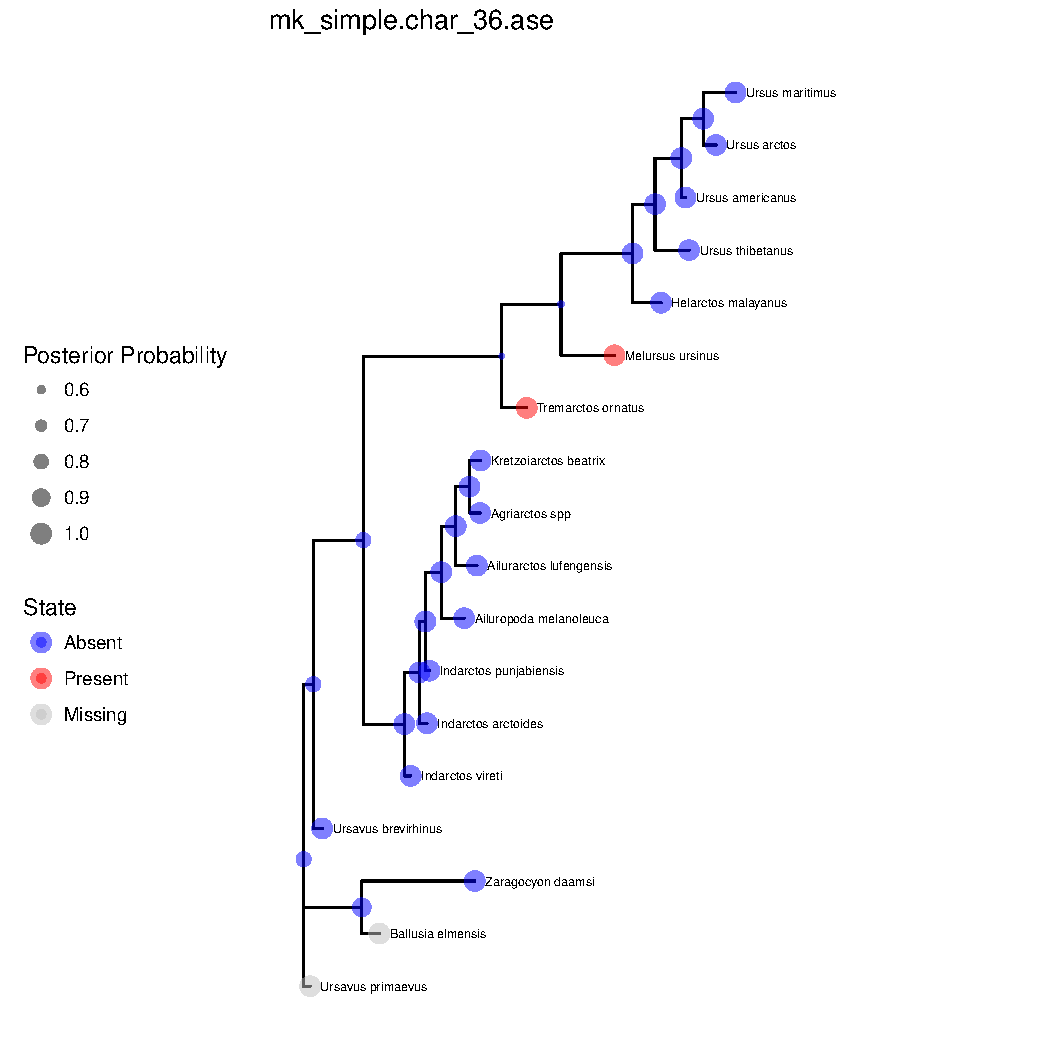
\includegraphics[width=0.92\textwidth,angle=0]{\ResourcePath figures/results/mk_simple_char_36_ase}
\caption{\small Ancestral state estimates assuming the uniform Mk model for character 36.}
\end{minipage}}
\label{fig:mk_simple_ase}
\end{figure}

\begin{figure}[h!]
\fbox{%
\begin{minipage}{\textwidth}\centering
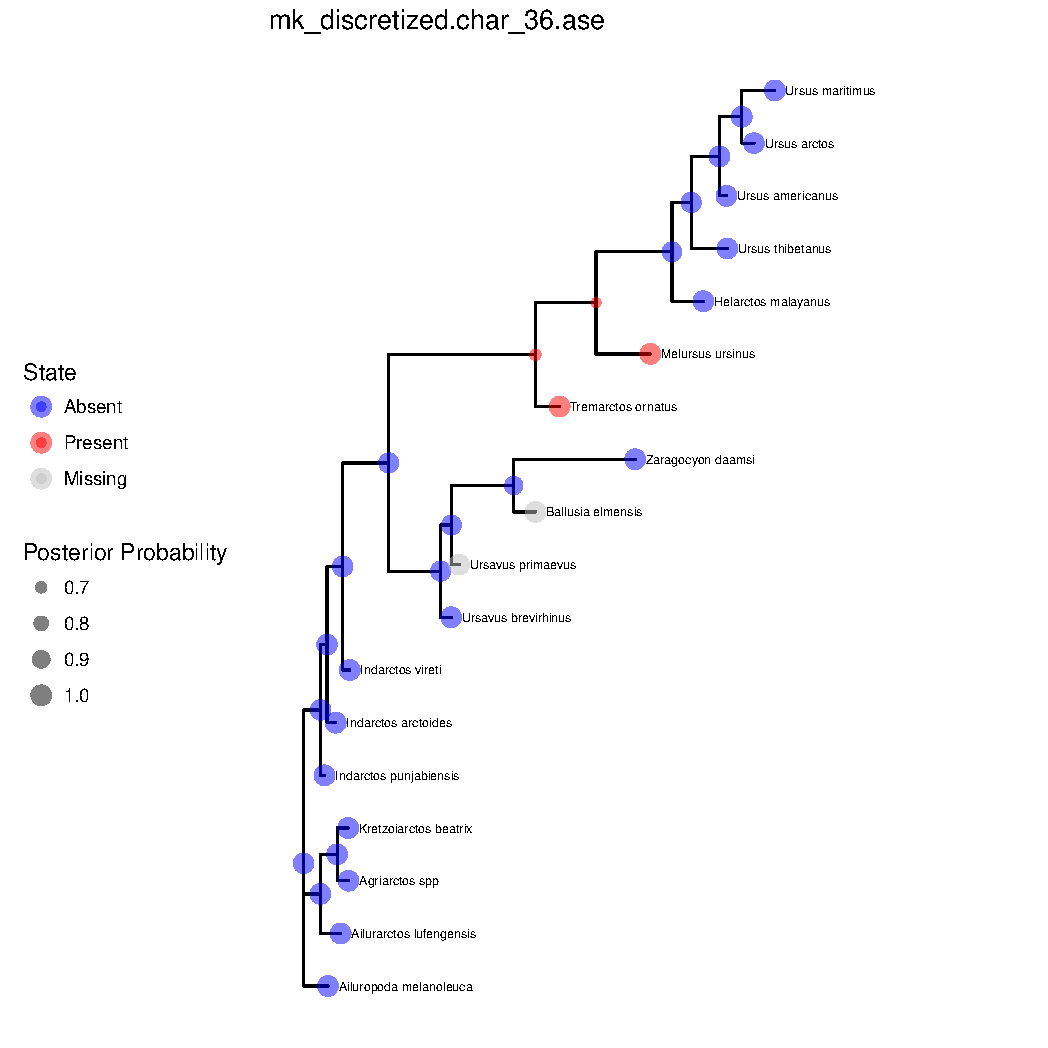
\includegraphics[width=0.92\textwidth,angle=0]{\ResourcePath figures/results/mk_discretized_char_36_ase}
\caption{\small Ancestral state estimates assuming the beta-discretized Mkv model for character 36.}
\end{minipage}}
\label{fig:mk_discretized_ase}
\end{figure}

Ancestral state estimate



\newpage
